% 2D Image with indices
% Author: Peter Steinbach
\documentclass[tikz]{standalone}
%\documentclass[dvisvgm]{standalone}
%\def\pgfsysdriver{pgfsys-tex4ht.def}
\usepackage{units}
\usepackage{tikz}
\usetikzlibrary{calc,math,trees,positioning,arrows.meta,chains,shapes.geometric,shapes.arrows,%
    decorations.pathreplacing,decorations.pathmorphing,shapes,%
    matrix,shapes.symbols,fit,backgrounds}

 \pgfdeclarelayer{back}
 \pgfsetlayers{background,back,main}


\makeatletter
\makeatother

\begin{document}
\begin{tikzpicture}

  \node (start) [draw=none] at(0,0) {};
  
  \foreach \i in {0,...,3}
           {
             %% \node (entity_\i) [rectangle,draw=black,very thick,minimum width=4.5cm,minimum height=1.cm,above] at($(start.east) + (4.75*\i,0)$) {};
             \node (thread_\i) [above,font=\huge,minimum width=5cm,] at($(start.east) + (8*\i,0)$) {$thread_\i$};
             \draw[dashed,thick] ($(thread_\i.north) + (-3.8,0)$) rectangle ($(thread_\i.north) + (3.8,-2)$);

   \foreach \j in {0,...,1}
           {
             \tikzmath{
               integer \x;
               \x = \i*4 + \j;
             }


             \node (devicet_\x) [rectangle,font=\LARGE,draw=gray,very thick,anchor=north,minimum height=.7cm,minimum width=.8cm] at($(thread_\i.west)+(\j*3,-.6)+(.5,0)$) {devices$[\x]$};
           }

           \tikzmath{
             integer \e;
             \e = \i+3;
           }

           \node (dots) [font=\Huge,very thick,right] at($(thread_\i.east) + (0,-1)$) {\dots};
         }

\end{tikzpicture}
\end{document}
